\documentclass[runningheads,a4paper]{llncs}

%
\usepackage{amssymb}
\usepackage{amsmath}
\usepackage{url}
\usepackage{graphicx}
\usepackage{multirow}
%
\newcommand{\argmin}[1]{\underset{#1}{\operatorname{arg}\operatorname{min}}\;}
\mathchardef\mhyphen="2D
\raggedbottom 
%
% Allow easy processing of labeled images in figures
\newcounter{lfigcounter}
\newenvironment{IonTab}{\begin{table}[htb]}{\end{table}}
\newenvironment{IonFig}{\setcounter{lfigcounter}{1}\begin{figure}} {\end{figure}}
\newenvironment{IonFigH}{\setcounter{lfigcounter}{1}\begin{figure}[h]}{\end{figure}}
\newenvironment{IonFigT}{\setcounter{lfigcounter}{1}\begin{figure}[!t]}{\end{figure}}
\newenvironment{IonFigB}{\setcounter{lfigcounter}{1}\begin{figure}[b]}{\end{figure}}
\def\ionbox#1{\makebox[#1]{(\alph{lfigcounter})}\stepcounter{lfigcounter}}
%
\begin{document}

\mainmatter  % start of an individual contribution

% first the title is needed
\title{An Image-based instantaneous phase estimation method for gating and temporal super-resolution of cardiac ultrasound}

% a short form should be given in case it is too long for the running head
\titlerunning{Image-based Phase Estimation Method for Cardiac Ultrasound}

% the name(s) of the author(s) follow(s) next
%
% NB: Chinese authors should write their first names(s) in front of
% their surnames. This ensures that the names appear correctly in
% the running heads and the author index.
%

% anonymous stuff
\author{*}
\authorrunning{*}   
\tocauthor{*}
\institute{*}

\maketitle

\begin{abstract}
Point-of-care low-cost hand-held ultrasound devices are emerging as an increasingly effective tool for rapid non-invasive visual assessment of cardiac structure and function on the bed-side. Their diagnostic value can be enriched further by coupling them with automated image analysis algorithms to accurately detect and quantify any cardiac abnormalities at the point-of-care potentially even in asymptomatic patients. However, a major challenge to this is the poor spatio-temporal resolution and high noise level of images obtained using these devices. In an effort to address this problem, we present a novel method for de-noising, gating, and temporal super-resolution of noisy low frame-rate periodic image sequences such as the ones obtained using low-cost hand-held cardiac ultrasound devices. We first leverage the inherent image-level redundancy in a periodic image sequence to decouple signal from noise using a low-rank + sparse decomposition algorithm. Next, we transform the complex high-dimensional periodic image sequence to a narrow-band 1D time series with the same periodicity characteristics using a novel strategy based on inter-frame similarity. Next, we decompose this time series use a season-trend decomposition method to obtain the heart-beat (season) and respiratory (trend) signals. Next, we use the Hilbert transform to estimate the instantaneous cardiac and respiratory phases of each frame to facilitate gating and super-resolution. Lastly, we use Nadarya-Watson kernel regression to construct an image manifold parameterized by intra-period phase which can then be sampled to reconstruct a de-noised single-period image sequence at a higher temporal-resolution. We demonstrate the utility and efficacy of our method both on synthetic data and on real image sequences of the beating heart acquired using a low-cost hand-held ultrasound device.
%\keywords{Denoising, Gating, Super-resolution, hand-held, Cardiac, Ultrasound}
\end{abstract}
\vspace{-0.5cm}
\section{Introduction}
\label{sec:intro}
Low-cost hand-held ultrasound devices are emerging as an increasingly effective tool for rapid non-invasive visual assessment of cardiac structure and function on the bed-side\cite{Wiley2014}. Their diagnostic value can be enriched further by coupling them with automated image analysis algorithms to accurately detect and quantify any cardiac abnormalities at the point-of-care potentially even in asymptomatic patients. However, a major challenge to this endeavour is the poor spatio-temporal resolution and high noise level of images obtained using these devices. Fortunately, in a periodic image sequence, such as the ones obtained in cardiac ultrasound, the expected temporal image-level redundancy/repetition can be exploited both for de-noising and super-resolution. These are precisely the problems that we intend to address here. Specifically, in this paper, we present a novel method for de-noising, gating and temporal super-resolution of noisy low frame-rate periodic image sequences such as the ones obtained using low-cost hand-held cardiac ultrasound devices. To our knowledge, there only one paper \cite{Makihara2011} that tries to address a similar problem on human gait sequences but the challenges posed by cardiac ultrasound videos that we intend to address here are different.
\vspace{-0.5cm}
\section{Method}
\label{sec:method}
%
In this section, we present the theory underlying the proposed method for de-noising, gating and temporal super-resolution of a noisy periodic image sequence. Specifically, we begin by describing how we de-noise a periodic image sequence using a low-rank $+$ sparse decomposition algorithm in Section \ref{sec:method:de-noising}. We then present a novel method for estimating the intra-period phase of each frame using the de-noised image sequence in Section \ref{sec:method:phase_estimation}. Finally, in Section \ref{sec:method:super-resolution}, we present a method that uses the phase-tagged image sequence to reconstruct a single-period video at higher-temporal resolution. 
%
\begin{IonFigT}
\centering
%
\makebox[1.5in]{Input}\makebox[1.5in]{LowRank}\makebox[1.5in]{Sparse}\\
\includegraphics[width=1.5in]{figures/VibratingCircle/imInput.png}
\includegraphics[width=1.5in]{figures/VibratingCircle/imLowRank.png}
\includegraphics[width=1.5in]{figures/VibratingCircle/imSparse.png}\\
\vspace{0.1cm}
\includegraphics[width=1.5in]{figures/VibratingCircle/imInput_MidX.png}
\includegraphics[width=1.5in]{figures/VibratingCircle/imLowRank_MidX.png}
\includegraphics[width=1.5in]{figures/VibratingCircle/imSparse_MidX.png}
\ionbox{4.5in}\\
\includegraphics[width=1.5in]{figures/SHeart2015-02-20-HRes-HFPS/Heart_20150220_151146/imInput.png}
\includegraphics[width=1.5in]{figures/SHeart2015-02-20-HRes-HFPS/Heart_20150220_151146/imLowRank.png}
\includegraphics[width=1.5in]{figures/SHeart2015-02-20-HRes-HFPS/Heart_20150220_151146/imSparse.png}\\
\vspace{0.1cm}
\includegraphics[width=1.5in]{figures/SHeart2015-02-20-HRes-HFPS/Heart_20150220_151146/imInput_MidX.png}
\includegraphics[width=1.5in]{figures/SHeart2015-02-20-HRes-HFPS/Heart_20150220_151146/imLowRank_MidX.png}
\includegraphics[width=1.5in]{figures/SHeart2015-02-20-HRes-HFPS/Heart_20150220_151146/imSparse_MidX.png}
\ionbox{4.5in}\\
%
\caption{Noise suppression using low-rank + sparse decomposition in (a) synthetic video of an expanding/contracting circle, and (b) real ultrasound video of beating heart. Images show temporal maximum intensity projections (top-row) and mid Y-T slices (bottom row) of the input (left), low-rank (middle), and sparse(right) videos.}
\label{fig:de-noising}
\end{IonFigT}
\vspace{-0.5cm}
\subsection{Noise suppression using low-rank $+$ sparse decomposition}
\label{sec:method:de-noising}
One of the main challenges for quantitative analysis of ultrasound image sequences in general, and the ones obtained using low-cost hand-held devices of interest to us in particular, is their high noise level. Fortunately, in a periodic image sequence, such as the ones seen in cardiac ultrasound, the expected image-level redundancy/repetition in time can be exploited to decouple the underlying signal from any distortions such as noise/occlusion if they do not affect the same set of pixels consistently over time. Inspired by their successful application to the problem of background-subtraction in surveillance videos\cite{Candes2009} by exploiting a similar kind of temporal redundancy, we use a low-rank $+$ sparse decomposition algorithm to suppress the noise in a periodic image sequence. Specifically, given a periodic image sequence $P = \{I_1, I_2, ..., I_n\}$ containing $n$ images with $m$ pixels each, we create an $m \times n$ matrix $D$ by stacking the images in the sequence as columns such that $i^{th}$ column of $D$ is a vectorized form of  image $I_i$ in the sequence $P$. We then decompose $D$ into the sum of a low-rank matrix $L$ and a sparse matrix $S$ by solving the following convex optimization problem using an augmented lagrangian approach:
\begin{equation}
\argmin{L,S}\left(\|L\|_{*} + \lambda \|S\|_1\right) 
\; s.t. \; D = L + S
\end{equation}
where $\| \cdot \|_*$ and $\| \cdot \|_1$ are the nuclear-norm and $\ell \mhyphen 1$ norm, respectively, and $\lambda > 0$ is a balancing parameter that we set to $1/{\sqrt{max\left(m,n\right)}}$. Due to the expected repetition of images across periods in a periodic image sequence and assuming that the noise/occlusions corrupting the images are sparse in time, the low-rank component $L$ approximates the noise-free image sequence and the sparse component $S$ captures the residual noise. Prior to low-rank + sparse decomposition, we apply a median filter to suppress any impulse noise and downsize the images if necessary to reduce computational time. For further analysis, we use the de-noised sequence of images $\{L_1, ..., L_n\}$ in the low-rank matrix $L$.
%
%
\begin{IonFigT}
\centering
%
\makebox[1.5in]{Similarity}\makebox[1.5in]{Similarity - Trend}\makebox[1.5in]{Similarity - Detrended}\\
\begin{tabular}{cc}
	\includegraphics[width=1.5in]{figures/VibratingCircle/simMat.png}
	\includegraphics[width=1.5in]{figures/VibratingCircle/simMat_Trend.png}
	\includegraphics[width=1.5in]{figures/VibratingCircle/simMat_Seasonal.png}
\end{tabular}\\
\ionbox{4.5in}\\
%
\begin{tabular}{cc}
	\begin{tabular}{c}
		\includegraphics[width=3.5in]{figures/VibratingCircle/ts_seasonal.png}\\
		\includegraphics[width=3.5in]{figures/VibratingCircle/ts_instaphase_comparison.png}
	\end{tabular}&	
	\begin{tabular}{c}
	
		\includegraphics[width=1.0in]		
			{figures/VibratingCircle/Input_est_phaseord_MidX.png}\\
		\makebox[1.0in]{Input}\\				
		\includegraphics[width=1.0in]		
			{figures/VibratingCircle/Lowrank_est_phaseord_MidX.png}\\		
		\makebox[1.0in]{Low-rank}				
	\end{tabular}			
\end{tabular}\\
\ionbox{3.5in}\ionbox{1.0in}\\
\caption{Intra-period phase estimation on synthetic expanding-contracting circle video: (a-left) Inter-frame similarity matrix, (a-mid) Trend computed using local regression, (a-right) Detrended similarity matrix, (b) Similarity profile of the row in the detrended similarity matrix with minimum spectral entropy (top) and the instantaneous intra-period phase (bottom) computed using the hilbert transform along with the groundtruth phaseto generate the input video, (c) Mid Y-T slice of input and low-rank videos with the frames ordered in ascending order of the estimated intra-period phase. Mean error in estimated phase against ground truth = 5.4 degrees.}
\label{fig:phase_estimation_synthetic}
\end{IonFigT}
%
%
\begin{IonFigT}
\centering
%
\makebox[1.5in]{Similarity}\makebox[1.5in]{Similarity - Trend}\makebox[1.5in]{Similarity - Detrended}\\
\begin{tabular}{cc}
	\includegraphics[width=1.5in]{figures/SHeart2015-02-20-HRes-HFPS/Heart_20150220_151146/simMat.png}
	\includegraphics[width=1.5in]{figures/SHeart2015-02-20-HRes-HFPS/Heart_20150220_151146/simMat_Trend.png}
	\includegraphics[width=1.5in]{figures/SHeart2015-02-20-HRes-HFPS/Heart_20150220_151146/simMat_Seasonal.png}
\end{tabular}\\
\ionbox{4.5in}\\
%
\begin{tabular}{cc}
	\begin{tabular}{c}
		\includegraphics[width=2.75in]{figures/SHeart2015-02-20-HRes-HFPS/Heart_20150220_151146/ts_seasonal.png}\\
		\includegraphics[width=2.75in]{figures/SHeart2015-02-20-HRes-HFPS/Heart_20150220_151146/ts_instaphase.png}
	\end{tabular}&	
	\begin{tabular}{c}
		\includegraphics[width=1.70in]		
			{figures/SHeart2015-02-20-HRes-HFPS/Heart_20150220_151146/Input_est_phaseord_MidX.png}\\
		\makebox[1.7in]{Input}\\				
	\end{tabular}			
\end{tabular}\\
\ionbox{2.75in}\ionbox{1.70in}\\
\caption{Intra-period phase estimation on cardiac ultrasound video: (a-left) Inter-frame similarity matrix, (a-mid) Trend computed using local regression, (a-right) Detrended similarity matrix, (b) Similarity profile of the row in the detrended similarity matrix with minimum spectral entropy (top) and the instantaneous intra-period phase (bottom) computed using the hilbert transform, (c) Mid Y-T slice of input and low-rank videos with the frames ordered in ascending order of the estimated intra-period phase.}
%
\label{fig:phase_estimation_heart}
\end{IonFigT}
%
\vspace{-0.5cm}
%
\subsection{Intra-period phase estimation of each frame}
\label{sec:method:phase_estimation}
%
To facilitate gating and super-resolution, we need to estimate the intra-period phase/position of each frame in the periodic image sequence. When compared to the widely studied problem of super-resolution using multiple low-resolution images of the same scene\cite{Nasrollahi2014}, the process of intra-period phase estimation in a periodic image sequence is analogous to alignment of the low-resolution images at a sub-pixel precision using a registration algorithm. While there have been numerous efforts for the estimation of instantaneous intra-period phase\cite{Lu2013} in periodic univariate time series data (wherein a single-variable is measured at each time point), we are not aware of any methods that tackle this problem in a multivariate setting which is the case with periodic image sequences wherein upto a million variables (intensities of pixels) could be measured at each time point. Our strategy was to find a way to simplify this seemingly complex multi-variate problem by transforming it into a univariate one and take advantage of existing methods to solve the problem at hand. To accomplish this, we compute the similarity/affinity between all pairs of frames in the given periodic image sequence containing $n$ images to create a matrix $A \in R^{n \times n}$ where in the element $A(i,j)$ is equal to the similarity between the $i^{th}$ and $j^{th}$ frames of the given sequence. In principle, any of the similarity metrics used in image registration algorithms can be chosen to quantify the similarity between a given pair of frames. Here in, we treat the images in the given sequence as points in high-dimensional space, apply principal component analysis (PCA) to reduce their dimensionality\cite{Bishop2006} such that 99\% of the total variance is covered, and use the $-ve$ distance in the PCA reduced subspace to quantify the similarity between any given pair of frames. Each row in the inter-frame similarity matrix $A$ can now be seen as a univariate time series that measures the similarity of the corresponding frame in the image sequence with all other frames. Additionally, for a periodic image sequence, we can expect them to be periodic provided that the corresponding frame is not significantly corrupted by distortions such as noise and changes in global illumination over time among others. To mitigate the potential problem of global illumintation changes over time, we detrend and extract the seasonal part of the time series corresponding to each row of $A$ by dividing it with the trend signal estimated using a locally-weighted regression algorithm called loess\cite{Cleveland1990}. Let $A_s$ be the matrix whose rows contain the seasonal part obtained by detrending the corresponding row in $A$. Next, we minimize the risk from noise, by finding the row $u(t)$ of $A_s$ whose power spectrum or periodogram has minimum entropy. In our experiments, the time series $u(t)$ was nearly sinusoidal in morphology with most of its energy in its power spectrum concentrated within a very narrow-band with the same periodicity characteristics as the image sequence it was derived from. Based on this observation, we decided to use its Hilbert transform \cite{Lu2013} to estimate the instantaneous intra-period phase  of each frame. Specifically, we compute the instantaneous phase $\phi(t) \in \left [  -\pi, \pi\right )$ of the time series $u(t)$ as follows:
\begin{equation}
\phi(t) = arctan \left( \frac{H_u(t)}{u(t)}\right)
\end{equation} 
where $H_u(t)$ is the Hilbert transform of $u(t)$. Lastly, we map the instantaneous phase $\phi(t)$ to the range $\left [  0, 1\right )$ which can then be used to obtain the intra-period phase of each frame.
%
%
\begin{IonFigT}
\centering
%
\includegraphics[height=0.9in]{figures/VibratingCircle/phase_derivative_error.png}
%
\includegraphics[height=0.8in]{figures/VibratingCircle/Input_Mag_2_linear_interpolation.png}
\includegraphics[height=0.8in]{figures/VibratingCircle/Input_Mag_4_linear_interpolation.png}
\includegraphics[height=0.8in]{figures/VibratingCircle/Input_Mag_8_linear_interpolation.png}
\hspace{.2in}
%
\includegraphics[height=0.8in]{figures/VibratingCircle/Input_Mag_2_kernel_regression.png}
\includegraphics[height=0.8in]{figures/VibratingCircle/Input_Mag_4_kernel_regression.png}
\includegraphics[height=0.8in]{figures/VibratingCircle/Input_Mag_8_kernel_regression.png}
\hspace{.2in}
%
\includegraphics[height=0.8in]{figures/VibratingCircle/Input_Mag_2_bspline_registration.png}
\includegraphics[height=0.8in]{figures/VibratingCircle/Input_Mag_4_bspline_registration.png}
\includegraphics[height=0.8in]{figures/VibratingCircle/Input_Mag_8_bspline_registration.png}
\hspace{.2in}
\\
\ionbox{1.0in}\ionbox{1.0in}\ionbox{1.0in}\ionbox{1.0in}
%
\\
%
%%\makebox[0.1in]{}
%\includegraphics[height=0.8in]{figures/SHeart2015-02-20-HRes-HFPS/Heart_20150220_151146/imHeartSuperRes_ValveMMode_4.png}
%\includegraphics[height=0.8in]{figures/SHeart2015-02-20-HRes-HFPS/Heart_20150220_151146/imHeartSuperRes_ValveMMode_8.png}
%\includegraphics[height=0.8in]{figures/SHeart2015-02-20-HRes-HFPS/Heart_20150220_151146/imHeartSuperRes_ValveMMode_16.png}\\
%\ionbox{3in}\makebox[0.1in]{}\ionbox{1in}
%
\caption{(a) Error with groundtruth of the phase difference between consecutive frames of phase-ordered synthetic video generated with varying levels of noise, (c-d) Mid YT slices of reconstructed one-period video of expanding-contracting circle at magnifications (left-right) of 2, 4, and 8 respectively}
\label{fig:super_resolution}
\end{IonFigT}
%
\vspace{-0.5cm}
%
\subsection{Reconstruction of one-period video at high temporal resolution}
\label{sec:method:super-resolution}
%
Once the intra-period phase of each frame has been estimated, it can be used (i) to facilitate the extraction of quantitative measurements from a desired part of the period, a process commonly referred to as gating, and (ii) to enable spatio-temporal super-resolution by considering the set of images within each period of a periodic image sequence as distinct observations of the same data. In this section, we present a method that uses a phase-tagged periodic image sequence to reconstruct a single-period video at a higher temporal resolution.  Given a de-noised periodic sequence $\{L_1, ..., L_n\}$ of $n$ images (with $m$ pixels each) along with their estimated intra-period phases $\{\phi_1, ..., \phi_n\}$, we first use Nadarya-Watson kernel regression\cite{Bishop2006} to construct a phase-parameterized image manifold in the form of a function $M(\phi): [0, 1) \to R^m $ that maps any intra-period phase $\phi$ to an image as follows:
\begin{equation}
M(\phi) = \frac{\sum_{i = 1}^{n} K(\phi, \phi_i) L_i}{\sum_{i = 1}^{n} K(\phi, \phi_i)} 
\end{equation}
where in we define the kernel $K$ using a gausssian with standard-deviation $\sigma$ equal to a multiple of the average distance between consecutive phases after sorting them. Note that, we account for the periodic nature of the intra-period phase whenever we measure distance between two phase values. A single-period video can now be reconstructed by sampling the manifold $M(\phi)$ at any desired resolution from the range $[0, 1)$ of intra-period phase. Note that the aformentioned process will facilitate temporal super-resolution only if the set of images observed in each distinct period of the given image sequence differ in intra-period phase by some non-zero amount less than its temporal sampling interval. Also, the amount of temporal super-resolution possible will depend both on the number of periods observed and the maximum amount by which one can expect the images to be perturbed in phase across observations. 
\vspace{-0.5cm}
\section{Results}
\label{sec:results}
We demonstrate the utility and efficacy of our method on synthetic videos of a periodically expanding-contracting circular membrane in Section~\ref{sec:results:vibrating_circle} and on real b-mode ultrasound videos of the beating human heart acquired in Section~\ref{sec:results:beating_heart}. 
\vspace{-0.5cm}
\subsection{Synthetic data: expanding-contracting circular membrane}
\label{sec:results:vibrating_circle}
In this section, we discuss the results obtained using the proposed method on synthetic videos of a circular membrane that expands and contracts periodically analogous to ultrasound videos of the beating heart in short-axis view. These videos are synthesized by  generating images of a circle whose radius various according to a sinusoidal function within a user-specified range of $[r_{min}, r_{max}]$. The images are smoothened using a gaussian filter of standard deviation $\sigma_m \times (r_{max} - r_{min})$ that determines the thickness of the circular membrane and corrupted by adding gaussian noise with standard deviation $\sigma_n$ . The frame length of the video is determined by number of cycles/periods of contraction-expansion $n_p$ and the number of samples within each period $n_s$. Lastly, to simulate phenomenon analogous to device-originated sampling noise and irregularities in the heart beat, we also perturb the sample phases by an amount of $\delta_p \in (0, 1]$ times the sampling interval before perturbation. Typical baseline values for the aforementioned parameters in our experiments are as follows: $r_{min} = 20, \; r_{max} = 50, \; \sigma_m = 0.1, \; \sigma_n = 0.1, \; n_p = 30, \; n_s = 20$. The intensity range of the images is set to $[0, 1]$. Fig.~\ref{fig:de-noising}(a) depicts the de-noising result obtained using low-rank $+$ sparse decomposition on a sample dataset as described in Section~\ref{sec:method:de-noising}. Observe the way in which most of the noise was absorbed by the sparse component. Fig.~\ref{fig:phase_estimation_synthetic} depicts the results of our phase estimation strategy described in Section~\ref{sec:method:phase_estimation}. Notice the periodic nature of images depicting the detrended inter-frame similarity matrix in Fig.~\ref{fig:phase_estimation_synthetic}(a) and the sinusoidal morphology of the similarity profile in Fig.~\ref{fig:phase_estimation_synthetic}(b) picked automatically for estimating the intra-period phase. Notice the continuity of the membrane in the Mid Y-T slice of the input and low-rank videos ordered by the estimated intra-period phase in Fig.~\ref{fig:phase_estimation_heart}. The mean and standard deviation of the mean error between the estimated and groundtruth intra-period phase accross five videos generated as described above was 7.56 and 1.346 degrees, respectively. Fig.~\ref{fig:super_resolution} shows the results of super-resolution at a series of increasing magnifications.
\vspace{-0.1cm}
\subsection{Real data: ultrasound video of beating heart}
\label{sec:results:beating_heart}
In this section, we discuss the results obtained using the proposed method on real b-mode ultrasound videos of the beating heart acquired using a hand-held ultrasound device. Each video was acquired at a frame rate of 36 frames per second with 14-17 heart beats during which the subject as asked to hold breath. Fig~\ref{fig:de-noising}(b) depicts the de-noising result obtained using low-rank $+$ sparse decomposition on a sample dataset as described in Section~\ref{sec:method:de-noising}. Notice that a significant percentage of the speckle noise was again absorbed by the sparse part. Fig~\ref{fig:phase_estimation_heart} depicts the results of our phase estimation strategy described in Section~\ref{sec:method:phase_estimation}. Again, notice the periodic pattern of the detrended inter-frame similarity matrix in Fig~\ref{fig:phase_estimation_heart}(a) and the near sinusoidal morphology of the similarity profile used to estimate the intra-period phase in Fig~\ref{fig:phase_estimation_heart}(b). Lastly, notice the continuity of the chamber wall over-time and its apparent expanding/contracting motion in Fig.~\ref{fig:phase_estimation_heart}(c).
\vspace{-0.5cm}
\section{Discussion and future work}
\label{sec:discussion}
The novel contributions of this paper are: (i) to leverage the inherent temporal image-level repetition/redundancy to decouple signal from noise in a noisy periodic image sequence, (ii) the proposed strategy based on inter-frame similarity to transform the multivariate problem of instantaneous intra-period phase estimation in a noisy complex high-dimensional periodic image sequence into a univariate problem to enable the use of existing methods in univariate time series analysis, (iii) using our method it may now become possible to gate or extract measurements from a desired portion of the cardiac cycle without using any other hardware thereby enriching the value of low-cost hand-held cardiac ultrasound devices at the point-of-care, and (iv) using our phase-estimation strategy the community can now translate the mature super-resolution technology in field of computer vision~\cite{Nasrollahi2014} to enhance the value of low-cost hand-held ultrasound devices even further. Having demonstrated a proof of concept of our ideas in this paper, our method has to be better evaluated on more datasets and especially on cardiac ultrasound videos of irregular heart beats. Lastly, since this paper deals with video analysis we encourage the reader to review the supplementary material for a better understanding of the proposed method.
\vspace{-0.5cm}
\bibliographystyle{splncs03}
\bibliography{library}
\end{document}







